\input /users/davidmcallester/icloud/tex/SlidePreamble
\input /users/davidmcallester/icloud/tex/preamble

\begin{document}

{\Huge

  \centerline{\bf TTIC 31230, Fundamentals of Deep Learning}

\bigskip

\centerline{David McAllester, Autumn  2023}

\vfill \vfill

\centerline{\bf Variational Auto-Encoders  (VAEs)}

\vfill \vfill

\slide{Fundamental Equations of Deep Learning}

\begin{itemize}
\item Cross Entropy Loss: $\Phi^* = {\color{red} \argmin_\Phi E_{(x,y)\sim \pop}\left[-\ln P_\Phi(y|x)\right]}$.

\vfill
\item GAN: $\gen^* = {\color{red} \argmax_{\gen} \min_{\disc} E_{i \sim \{-1,1\}, y \sim P_i}\left[-\ln P_{\disc}(i|y)\right]}$.

\vfill
\item VAE (including diffusion models)
\begin{eqnarray*}
& & \pri^*,\gen^*,\enc^* \\
\\
& = & {\color{red} \argmin_{\pri,\gen,\enc}\;E_{y \sim \pop,z \sim P_\enc(z|y)}\left[ - \ln \frac{P_\pri(z)P_\gen(y|z)}{P_\enc(z|y)}\right]}
\end{eqnarray*}
\end{itemize}

\slide{Generative AI for Continuous Data: VAEs}
A variational autoencoder (VAE) is defined by three parts:

\vfill
\begin{itemize}
\item An encoder distribution $P_\enc(z|y)$.

\vfill
\item A ``prior'' distribution $P_\pri(z)$

\vfill
\item A generator distribution $P_\gen(y|z)$
\end{itemize}

\vfill
VAE generation uses $P_\pri(z)$ and $P_\gen(y|z)$ (like a GAN).

\vfill
VAE training uses a ``GAN inverter'' $P_\enc(z|y)$.

\slide{Fixed Encoder Training}
$$\pri^*,\gen^* = \argmin_{\pri,\gen}\;E_{y \sim \pop(y),z \sim \enc(z|y)}\left[-\ln P_\pri(z)P_\gen(y|z)\right]$$

\vfill
This is cross-entropy loss from $\pop(y)P_\enc(z|y)$ to $P_\pri(z)P_\gen(y|z)$

\vfill
Universality gives

{\color{red} $$P_{\pri^*}(z)P_{\gen^*}(y|z) = \pop(y)P_\enc(z|y)$$}

\vfill
Hence sampling from $P_{\pri^*}(z)P_{\gen^*}(y|z)$ samples $y$ from the population.


\slide{Degrees of Freedom}

{\color{red} $$P_\pri(z)P_\gen(y|z) = \pop(y)P_\enc(z|y)$$}

\vfill
Any joint distribution on $(y,z)$ with the desired marginal on $y$ optimizes the bound.

\slide{Bayesian Encoder Training}

We consider the case of a probabilitic model with a small number of parameters (by deep learning standards).

\vfill
For example a Gaussian mixture model (GMM) or a probabilistic context free grammar (PCFG).

\vfill
Such models impose a strong structural constraint and are far from universal.

\vfill
For such models we clearly need to train the encoder.  More generally, training the encoder can improve the model
(reduce an upper bound on $H(y)$).


\slide{Training the Encoder (the GAN Inverter)}

Define the ELBO loss as follows (acronym described later).
\begin{eqnarray*}
{\cal L}(y,z) & = & - \ln \frac{P_\pri(z)P_\gen(y|z)}{P_\enc(z|y)}
\end{eqnarray*}

\vfill
Recall cross-entropy loss: {\color{red} $H(y) \leq E_{y\sim \pop} \left[ -\ln P_\Phi(y)\right]$}

\vfill
We will show
{\color{red} $H(y) \leq E_{y \sim \pop,z \sim P_\enc(z|y)}\;{\cal L}(y,z)$}

\slide{A Bayesian Interpretation}

VAEs were originally motivated by a Bayesian interpretation:

\vfill
\begin{itemize}
\item $P_\pri(z)$ is the Bayesian prior on hypothesis $z$.

\vfill
\item $P_\gen(y|z)$ is the propability of the ``evidence'' $y$ given hypothesis $z$.

\vfill
\item $P_\enc(z|y)$ is a model approximating the Bayesian posterior on hypothesis $z$ given evidence $y$.
\end{itemize}

\vfill
The Bayesian motivation is to train $P_\enc(z|y)$ to approximate Bayesian inference.

\slide{Bayesian Interpretation}
{\huge
\begin{eqnarray*}
H(\pop) & \leq & E_{y\sim \pop} \left[-\ln P_{\pri,\gen}(y)\right] \\
\\
\ln P_{\pri,\gen}(y) & =  & \ln \frac{P_{\pri}(z)P_\gen(y|z)}{P_{\pri,\gen}(z|y)} \\
\\
\\
& = & E_{z \sim P_\enc(z|y)}\left[\ln \frac{P_{\pri}(z)P_\gen(y|z)}{P_\enc(z|y)}\right] + KL(P_\enc(z|y),P_{\pri,\gen}(z|y)) \\
\\
\\
& \geq & E_{z \sim P_\enc(z|y)}\left[\ln \frac{P_{\pri}(z)P_\gen(y|z)}{P_\enc(z|y)}\right] \\
\end{eqnarray*}
}
A Bayesian thinks of $y$ as ``evidence'' for hypothesis $z$.

\vfill
{\color{red} $E_{z\sim P_\enc(z|y)}[-{\cal L}(y,z)]$} is called {\color{red} the evidence lower bound (ELBO)}.


\slideplain{Expectation Maximization (EM)}

Expectation Maximimization (EM) applies in the (highly special) case where the exact posterior $P_{\pri,\gen}(z|y)$ is samplable and computable.
EM alternates exact optimization of $\enc$ and the pair $(\pri,\gen)$ in:
$$\mbox{VAE:}\;\;\;\;\;\;\; {\color{red} \pri^*,\gen^*} = \argmin_{\color{red} \pri,\gen} \min_{\color{red} \enc} E_{y,\;z \sim P_{\color{red} \enc}(z|y)}\;\;- \ln \frac{P_{\color{red} \pri,\gen}(z,y)}{P_{\color{red} \enc}(z|y)}$$

\vfill
$$\mbox{EM:}\;\;\;\;\;\; {\color{red} \pri^{t+1},\gen^{t+1}} =  \argmin_{\color{red} \pri,\gen}\;\;\;\;E_{y,\;z \sim P_{\color{red} \pri^t,\gen^t}(z|y)}\; - \ln P_{\color{red} \pri,\gen}(z,y)$$

\vfill
\centerline{\hspace{1em} Inference \hspace{6em} Update \hspace{2.5em}~}
\centerline{(E Step) \hspace{6em} (M Step) ~}
\centerline{ $P_\enc(z|y) = P_{\pri^{\color{red} t},\gen^{\color{red} t}}(z|y)$ \hspace{2.5em} Hold $P_\enc(z|y)$ fixed \hspace{0em}~}

\slide{Posterior Collapse}


{\color{red} $$P_\pri(z)P_\gen(y|z) = \pop(y)P_\enc(z|y)$$}

\vfill
Any joint distribution on $(y,z)$ with the desired marginal on $y$ optimizes the bound.

\vfill
This allows the prior and the encoder (the posterior) to both degenerate to having no mutual information with $y$.

\vfill
This often happens in language modeling.

\slide{The Reparameterization Trick}

$$\enc^* = \argmin_{\enc}\;\;E_{y\sim \pop(y),{\color{red} z\sim P_\enc(z|y)}}\;\left[- \ln \frac{P_\pri(z)P_\gen(y|z)}{P_\enc(z|y)}\right]$$

\vfill
Gradient descent on the encoder parameters must take into account the fact that we are sampling from the encoder.

\vfill
To handle this we sample noise $\epsilon$ from a fixed noise distribution and replace $z$ with a determinstc function $z_\enc(y,\epsilon)$

\vfill
$$\enc^*,\pri^*,\gen^* = \argmin_{\enc,\pri,\gen}\;\;E_{y,{\color{red} \epsilon,z=\hat{z}_\enc(y,\epsilon)}}\;\left[- \ln \frac{P_\pri(z)P_\gen(y|z)}{P_\enc(z|y)}\right]$$

\slide{The Reparameterization Trick}

$$\enc^*,\pri^*,\gen^* = \argmin_{\enc,\pri,\gen}\;\;E_{y,{\color{red} \epsilon,z=\hat{z}_\enc(y,\epsilon)}}\;\left[- \ln \frac{P_\pri(z)P_\gen(y|z)}{P_\enc(z|y)}\right]$$

\vfill
To get gradients we must have that $\hat{z}_\enc(y,\epsilon)$ is a differentiable function of the encoder parameters.

\vfill
Optimizing the encoder is tricky for discrete $z$.  Discrete $z$ is handled effectively in EM algorithms and general vector quantization (VQ) methods.

\slide{The KL-divergence Optimization}
{\huge
For Gaussian Models we have
\vfill
\begin{eqnarray*}
{\cal L}(y) & = & E_{z \sim P_\enc(z|y)}\left[ - \ln \frac{P_\pri(z)P_\gen(y|z)}{P_\enc(z|y)}\right] \\
\\
& = & {\color{red} KL(P_\enc(z|y),P_\pri(z))} + E_{z \sim P_\enc(z|y)}\left[- \ln P_\gen(y|z)\right] \\
\\
\\
&=& {\color{red} \frac{||\hat{z}_\enc(y) - \hat{z}_\pri||^2}{2\sigma^2}} + E_\epsilon\;\frac{||y - \hat{y}_\gen(\hat{z}_\enc(y,\epsilon))||^2}{2\sigma^2}
\end{eqnarray*}

\vfill
A closed-form expression for the KL term avoids sampling noise.
}

\slide{Hierarchical VAEs}


\centerline{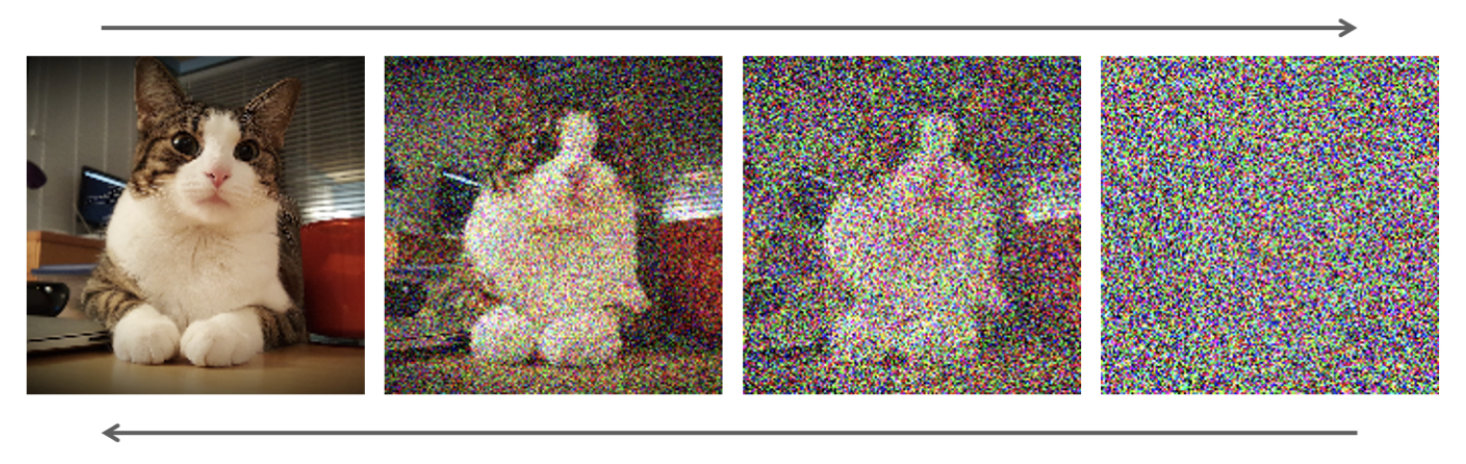
\includegraphics[width = 7in]{\images/DiffSequence}}

\vfill
{\huge
\centerline{{\color{red} [Sally talked to John]} $\stackrel{\rightarrow}{\leftarrow}$ {\color{red} [Sally talked to]}
$\stackrel{\rightarrow}{\leftarrow}$ {\color{red}[Sally talked]} $\stackrel{\rightarrow}{\leftarrow}$ {\color{red}[Sally]} $\stackrel{\rightarrow}{\leftarrow}$ {\color{red} []}}
}

\vfill
\centerline{$y \stackrel{\rightarrow}{\leftarrow} z_1  \stackrel{\rightarrow}{\leftarrow} \cdots \stackrel{\rightarrow}{\leftarrow} z_N$}

\slide{Hierarchical VAEs}
\centerline{$y \stackrel{\rightarrow}{\leftarrow} z_1  \stackrel{\rightarrow}{\leftarrow} \cdots \stackrel{\rightarrow}{\leftarrow} z_N$}

\vfill
{\bf Encoder}: $\pop(y)$, $P_\enc(z_1|y)$, and $P_\enc(z_{\ell+1}|z_\ell)$.


\vfill
{\bf Generator}: $P_\pri(z_N)$, $P_\gen(z_{\ell-1}|z_\ell)$, $P_\gen(y|z_1)$.

\vfill
The encoder and the decoder define distributions $P_\enc(y,\ldots,z_N)$ and $P_\gen(y,\ldots,z_N)$ respectively.


\slide{Hierarchical VAEs}

\centerline{$y \stackrel{\rightarrow}{\leftarrow} z_1  \stackrel{\rightarrow}{\leftarrow} \cdots \stackrel{\rightarrow}{\leftarrow} z_N$}

\vfill
\begin{itemize}
\item autoregressive models

\vfill
\item diffusion models
\end{itemize}


\slide{Hierarchical (or Diffusion) ELBO}

{\Large
\begin{eqnarray*}
H(y) & = & E_\enc\left[- \ln\frac{P_\enc(y)P_\enc(z_1,\ldots,z_N|y)}{P_\enc(z_1,\ldots,z_N|y)}\right]\\
  \\
  \\
  & = & E_\enc\left[ - \ln\frac{P_{\color{red} \enc}(y|z_1)P_{\color{red} \enc}(z_1|z_2)\cdots P_{\color{red} \enc}(z_{N-1}|z_N)P_{\color{red} \enc}(z_N)}
  {P_\enc(z_1|z_2,y)\cdots P_\enc(z_{N-1}|z_N,y)P_\enc(z_N|y)}\right] \\
   \\
   \\
  & {\color{red} \leq} & E_\enc\left[ - \ln\frac{P_{\color{red} \gen}(y|z_1)P_{\color{red} \gen}(z_1|z_2)\cdots P_{\color{red} \gen}(z_{N-1}|z_N)P_{\color{red} \gen}(z_N)}
  {P_\enc(z_1|z_2,y)\cdots P_\enc(z_{N-1}|z_N,y)P_\enc(z_N|y)}\right] \\
\\
\\
 & = & \left\{\begin{array}{l}E_\enc\;[-\ln P_\gen(y|z_1)]
                             \\ \\ + \sum_{i=2}^N  \; E_\enc\; KL(P_\enc(z_{i-1}|z_i,y),\;P_\gen(z_{i-1}|z_i)) \\
                             \\ + E_\enc\; KL(P_\enc(Z_N|y),p_\gen(Z_N))\end{array}\right.
\end{eqnarray*}
}

\slide{END}

\end{document}
